\documentclass{article}
\newcommand{\Red}[1]{\textcolor{black}{#1}}
\usepackage{graphicx,amssymb}
\usepackage{amsmath}
\usepackage{cases}
\usepackage{float}
\usepackage{listings}
\usepackage{times}
\usepackage{tikz}
\usepackage{epic}
%\usepackage{pstcol}
\usepackage{titlesec}
\usepackage{geometry}
%\usepackage{amsthm}
\usepackage{bm}
\usepackage{stmaryrd}
%\usepackage{subfigure}
\usepackage{indentfirst}
\usepackage{xcolor}
\usepackage{epstopdf}
\usepackage{enumerate}
\usepackage{enumitem}
\usepackage{hyperref}
\usepackage{makecell}
\usepackage{graphicx}
\usepackage{subcaption}
\usepackage{mwe}
\newcommand{\vertii}[1]{\lVert#1\rVert}


%\title{Using Neural Networks on Multigrid Methods for Diffusion Equations}
%\vspace{20mm}
%Master Project Report
%\author{Tsz Fung Yu }
%\date{August 2023}

\begin{document}

%\maketitle

\begin{titlepage}
   \begin{center}
       \vspace*{3cm}

        \Large
       \textbf{Transfer Operators with Neural Networks}
            
       \vspace{1.5cm}
       
        \Large
       \textbf{Tsz Fung Yu}

    

       \vfill
            
       
            
       \vspace{0.8cm}
            
       Warwick Mathematics Institute\\
       August 2025
            
   \end{center}
\end{titlepage}
 \newpage
\section{Introduction}



\section{Learning transition paths through neural operator}

In this part, we turn our focus on using neural networks to solve a PDE directly, rather than using neural network as a part of an existing numerical method. \\


Suppose we have two disjoint sets $A$ and $B$ in a 2D area. A particle in between in experiencing both diffusion and advection in the area. We would like to consider the probability that what pathway it will take. These probabilities are called transition paths. \\

These movements are usually modeled with a Markov process $\left\{X_{t}\right\}_{t \in T} \subseteq \Omega \subset \mathbb{R}^{n}$ governed by a stochastic differential equation (SDE) of the form
$$
\mathrm{d} X_{t}=b\left(X_{t}, t\right) \mathrm{d} t+\sigma\left(X_{t}, t\right) \mathrm{d} W_{t}
$$
where $W_{t}$ is the standard Brownian motion in $\mathbb{R}^{n}, b$ is the velocity field and $\sigma$ is the diffusion coefficient. In this paper we consider stochastic processes $\left\{X_{t}\right\}_{t \in T}$ in a 2D domain $\Omega$ that is vertically periodic and bounded on the left and right by the sets $A$ and $B$. Figure shows an example domain. 
\begin{figure}[ht]
  \centering
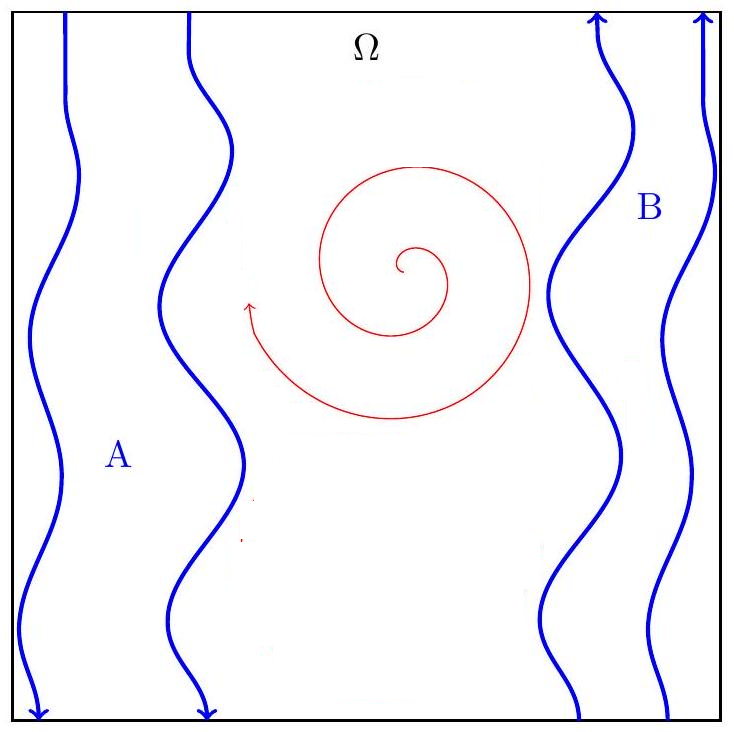
\includegraphics[width=0.5\linewidth]{turbulant.png}
  \caption{Turbulent flow diagram. The domain $\Omega$ lies between sets $A$ and $B$.}
  \label{fig:turbulant}
\end{figure}
The goal is to model a turbulent flow in a fluid, which we aim to predict what is the most likely transition path that a particle starting in set $A$ will go to get to set $B$. For simplicity, we assume that the turbulant velocity field $b$ is in equilibrium, and assume that no other factors affect the diffusion, thus taking $\sigma\left(X_{t}\right)=\sqrt{2} I_{2}$, where $I_{2}$ is the identity matrix. We then arrive at the following SDE
$$
\mathrm{d} X_{t}=b\left(X_{t}\right) \mathrm{d} t+\sqrt{2} I_{2} \mathrm{~d} W_{t}
$$
 The SDE above is related to the Fokker-Planck equation, which each random variable $X_{t}$ has a probability density function $\rho$ that satisfies the following Fokker-Planck equation
$$
\partial_{t} \rho=\nabla \cdot(-b(\boldsymbol{x}) \rho+\nabla \rho)
$$

 When $\partial_{t} \rho=0$ we call the solution $\rho(x)$ the steady probability density function. \\

Given a set $S$ and a time $t$ we define the hitting times
$$
\tau_{S}:=\inf \left\{s>0 \mid X_{s} \in S\right\}, \quad \tau_{S}^{+}:=\inf _{s>0}\left\{s \mid X_{t+s} \in S\right\}, \quad \tau_{S}^{-}:=\sup _{s<0}\left\{s \mid X_{t+s} \in S\right\}
$$
These represent the first time a stochastic process reaches the set $S$, the next time we reach $S$ in the future, and the last time we hit $S$ in the past. \\

We are interested in the probability that the stochastic process which hit $A$ from the past, and then reach $B$ later. We define the forward and backward committor functions, $q^{+}$and $q^{-}$ as follows:
$$
q^{+}(x)=P\left(\tau_{B}^{+}<\tau_{A}^{+} \mid X_{t}=\boldsymbol{x}\right), \quad q^{-}(x)=P\left(\tau_{B}^{-}<\tau_{A}^{-} \mid X_{t}=\boldsymbol{x}\right)
$$

These are conditional probability densities which can be found by solving the Dirichlet problems
$$
\left\{\begin{array}{cl}
L q^{+}(\boldsymbol{x})=0 & \forall \boldsymbol{x} \in \Omega \\
q^{+}(\boldsymbol{x})=0, & \forall \boldsymbol{x} \in \partial A \\
q^{+}(\boldsymbol{x})=1, & \forall \boldsymbol{x} \in \partial B
\end{array}\right.
$$
and
$$
\begin{cases}\bar{L} q^{-}(\boldsymbol{x})=0, & \forall \boldsymbol{x} \in \Omega \\ q^{-}(\boldsymbol{x})=1, & \forall \boldsymbol{x} \in \partial A \\ q^{-}(\boldsymbol{x})=0 & \forall \boldsymbol{x} \in \partial B\end{cases}
$$
where $\bar{L}$ is the generator of the reverse Markov process given by
$$
\bar{L} q^{-}:=\Delta q^{-}+b^{R} \cdot \nabla q^{-}, \quad \text { with } b^{R}(\boldsymbol{x})=-b(\boldsymbol{x})+\frac{2}{\rho(\boldsymbol{x})} \nabla \cdot(a(\boldsymbol{x}) \rho(\boldsymbol{x}))
$$
Of particular interest is the probability density of reactive trajectories
$$
\rho_{\text {react }}(\boldsymbol{x})=q^{-}(\boldsymbol{x}) \rho(\boldsymbol{x}) q^{+}(\boldsymbol{x})
$$
which concerns the probability of last hitting $A$, being at position $\boldsymbol{x}$ currently, and reaching $B$ next. 
This quantity peaks at regions where trajectories transitioning
from $A$ to $B$ spend most of their time. They are therefore called
dynamical bottlenecks. \\

It would be interesting to compute dynamical bottlenecks for various
stochastic models, as they are the region where the most important
difficulty is overcome for a transition. For example, one could consider
a climate model that describes ice-albedo-feedback of earth, or the
metastable gulf-stream in the north atlantic, and analyze which regions
of state space are the important bottleneck for a snowball earth or for
a gulf-stream shutdown. \\

The problem is that one needs to solve the advection-diffusion equations as above,
which are very high dimensional PDEs for even moderate-dimensional
original SDEs. In particular, if the SDE is in $\R^n$, then the advection-diffusion equations is an
$n$-dimensional PDE, which is difficult to solve with traditional methods. \\

In this part, we would like to learn the action of the generator using operator learning, and thus solve these equations for unseen boundary conditions. 

\subsection{Literature review}

[Not done for now, but basically paper work. Need reference for later parts too. I use [] to indicate a reference is needed.]
\subsection{Methods}

\subsubsection{Operator Learning}

Operator learning is used to learn the mapping between two infinite dimensional function spaces $\mathcal{U}$ and $\mathcal{V}$. We use the notation of Kovachki et al. [] and consider separable Banach spaces of vector valued functions:
$$
\begin{array}{ll}
\mathcal{U}=\left\{u: \mathfrak{D}_{x} \rightarrow \mathbb{R}^{d_{i}}\right\}, & \mathfrak{D}_{x} \subseteq \mathbb{R}^{d_{x}}, \\
\mathcal{V}=\left\{v: \mathfrak{D}_{y} \rightarrow \mathbb{R}^{d_{o}}\right\}, & \mathfrak{D}_{y} \subseteq \mathbb{R}^{d_{y}} .
\end{array}
$$

Operator learning is a gereralization of neural networks, which is introduced in the earlier part of the paper. Neural operators consists of different types of layers, like neural network. The input layer for a neural operator is a function $f \in \mathcal{U}$. In practice, the input layer is usually a finite representation of the desired function, like discretised point evaluation. The output layer is a function $v \in \mathcal{V}$. The layer in between , namely layer $i$, is the integral of a kernel $K^{(i)}$ on a compact domain $\Omega_{i} \subset \mathbb{R}^{d_{i}}$ against the output of the previous layer $v_{i}$. A non-linear bias function $b_{i} \in \mathbb{R}^{d_{i}}$ is then added to the integral and an activation function $\sigma$ is applied to this expression to get input for the next layer, $v_{i+1}$. This process can be written as
$$
v_{i+1}(x)=\sigma\left(\int_{\Omega_{i}} K^{(i)}(x, y) v_{i}(y) \mathrm{d} y+b_{i}(x)\right), \quad x \in \Omega_{i+1}
$$

Compared with neural network, the integration inside the kernel is a continuous analogue of the matrix multiplication in neural network and different types of kernels correspond to different types of matrices. We want to learn the bias and kernel functions and optimize each layer, just like in neural network setting. The learning itself is basically the same with neural network, with supervised learning and back propagation of errors. Refer to the previous section for more on that. We would like to focus on the main difference here.
The main obstacle in the learning is about approximating the kernel and the integral. Different methods of approximation in the kernal leads to different neural operator structures. \\

Below we introduce some structures of neural operator that is used in our paper.

\subsubsection{DeepONet}

A DeepONet is introduced by Lu et.al as a very first operator learning that successfully solves nonlinear PDEs []. It is a two-part deep learning network consisting of a branch network and a trunk network. The branch net encodes the operator's input functions $f$ into compact, fixed-size latent vectors $b_1\left(f\left(x_1\right), \ldots, f\left(x_m\right)\right), \ldots, b_p\left(f\left(x_1\right), \ldots, f\left(x_m\right)\right)$, where $\left\{x_i\right\}_{i=1}^m$ are the sensor points at which the input functions are evaluated. The trunk net decodes these latent vectors to produce the final output function at the location $y$ as
$$
\mathcal{N}(f)(y)=\sum_{k=1}^p b_k\left(f\left(x_1\right), \ldots, f\left(x_m\right)\right) t_k(y) .
$$

A schematic of a deep operator network is given in Figure \ref{fig:deepo} [Now I just copy the figure from other paper[], which will be changed]. 
\begin{figure}[ht]
  \centering
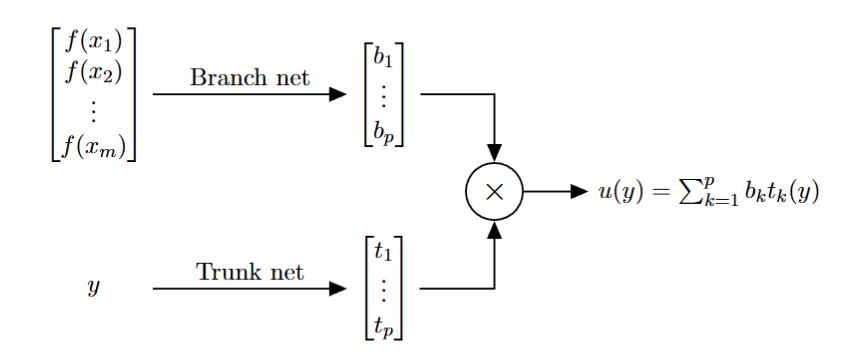
\includegraphics[width=0.7\linewidth]{deeponet_fig.png}
  \caption{DeepONet structure. Consists of the branch network and trunk network.}
  \label{fig:deepo}
\end{figure}
The defining feature of DeepONets is their ability to handle functional input and output, thus enabling them to learn a wide array of mathematical operators effectively. The neural networks of the branch and trunk are not really specified, so they can be changed to other structures of neural network to adapt to different types of problems. 

\subsubsection{Fourier Neural Operator}

The Fourier neural operator (FNO) architecture was introduced by Li et al []. The idea behind the FNO is to choose translation invariant kernels in the neural layer in (8) of the form
$$
K^{(i)}(\boldsymbol{x}, \boldsymbol{y})=k^{(i)}(\boldsymbol{x}-\boldsymbol{y}),
$$
where the integration of the $k^{(i)}$ is now a convolution operation. Convolution in the spacial domain can be computed with pointwise multiplication in the Fourier domain, and the resulting integral operation is 
$$
\int_{\Omega_{i}} k^{(i)}(\boldsymbol{x}-\boldsymbol{y}) v_{i} \mathrm{~d} y=\mathcal{F}^{-1}\left(\mathcal{F}\left(k^{(i)}\right) \mathcal{F}\left(v_{i}\right)\right)(\boldsymbol{x})
$$
where $\mathcal{F}$ is the Fourier transform and $\mathcal{F}^{-1}$ the inverse Fourier transform, defined for $f: \Omega_{i} \rightarrow \mathbb{R}^{d_{c}}$ by
$$
(\mathcal{F} f)_{j}(\boldsymbol{k})=\int_{\Omega_{i}} f_{j}(\boldsymbol{x}) e^{-2 i \pi \boldsymbol{x} \cdot \boldsymbol{k}} \mathrm{~d} \boldsymbol{x}, \quad\left(\mathcal{F}^{-1} f\right)_{j}(\boldsymbol{x})=\int_{\Omega_{i}} f_{j}(\boldsymbol{x}) e^{2 i \pi \boldsymbol{x} \cdot \boldsymbol{k}} \mathrm{~d} \boldsymbol{k}
$$
for $j=1, \ldots, d_{c}$. 
The Fourier transform takes a function from the physical space to the frequency domain, where $\boldsymbol{k}$ is the wave number. The transformation can be computed efficiently by the Fast Fourier Transform (FFT) technique, which reduces the time complexity of the transform operation from the usual $O(n^2)$ to $O(n \log n)$, where $n$ is the number of grid point evaluations for one instance of a PDE. We can suit the FFT conditions by letting the kernel to be a periodic function. It can be parameterised using the weight vector, $\gamma$, which are the Fourier coefficients. We truncate $\gamma$ to a band of Fourier modes which acts as a discretisation. and $\gamma$ is optimized during the training. The maximum number of Fourier modes $k_{\text {max }}$ is often chosen to be less than 16 as PDEs with smooth solutions experience rapid decay in Fourier coefficients. The bias term $b_{i}$ in the neural layer is used to add non-periodicity to the solutions [].

We can define the FNO architecture as follows:
$$
\begin{aligned}
\Psi_{\mathrm{FNO}}(u ; \theta) & =\mathcal{Q} \circ \mathcal{L}_{L} \circ \cdots \circ \mathcal{L}_{2} \circ \mathcal{L}_{1} \circ \mathcal{R}(u ; \theta), \quad \forall u \in \mathcal{U}, \\
\mathcal{L}_{l}(v)(\boldsymbol{x} ; \theta) & =\sigma\left(W_{l} v(\boldsymbol{x})+b_{l}+\mathcal{K}(v)\left(\boldsymbol{x} ; \gamma_{l}\right)\right), \quad \forall l \in[1, L] .
\end{aligned}
$$

\subsubsection {Convolution Neural Operator}
[In testing now, not sure if it works or not]

\subsubsection{Fokker-Planck equation}

In this section we derive the Fokker-Planck equation that we ultimately want to solve. \\ 

In its most general form the Fokker-Planck equation[] that describes the probability density of $X_{t}$ in the SDE (2) takes the form
$$
\partial_{t} u=\sum_{i, j=1}^{d} a_{i j} \frac{\partial^{2} u}{\partial x_{i} \partial x_{j}}+b \cdot \nabla u
$$
In our case, $a=I_{2}$ is the diffusion coefficient and $b(\boldsymbol{x}): \mathbb{R}^{d} \rightarrow \mathbb{R}$ is the velocity field. This represents the probability density of a stochastic process. The equation is also known as the forward or backward Kolmogorov equation depending on whether the sign in front of $b(\boldsymbol{x})$ is negative or positive respectively. We assume that the velocity field is divergence-free, which is $b \cdot \nabla u=0$. From here on let $\boldsymbol{x}=(x, y)$. We assume that our domain $\Omega$ is periodic in $y$ so that no mass can escape our system. When $\partial_{t} u$ is set to 0 we call the equation steady. \\

The existence and uniqueness of both the forward and backward Kolmogorov equation is stated in [], with the assumption of $b \in L^\infty$. We omit the proof in here, and refer the details to the book [].

\subsubsection{The Forward Committor Function}

The forward committor function $q^{+}(\boldsymbol{x})$, is the probability that a stochastic process will reach set next $B$ if it is at point $\boldsymbol{x} \in \Omega$. This function is the solution to the following backward Kolmogorov equation
$$
\begin{cases}\Delta q^{+}(\boldsymbol{x})+b(\boldsymbol{x}) \cdot \nabla q^{+}(\boldsymbol{x})=0, & \boldsymbol{x} \in \Omega \backslash(A \cup B) \\ q^{+}(\boldsymbol{x})=0, & \boldsymbol{x} \in \partial A \\ q^{+}(\boldsymbol{x})=1, & \boldsymbol{x} \in \partial B \\ \left.q^{+}\right|_{y=0}=\left.q^{+}\right|_{y=1}, & \text { (periodic boundaries). }\end{cases}
$$




\subsubsection{The Steady Probability Density Function}

The steady, or stationary, probability density function $\rho(\boldsymbol{x})$ solves the following steady forward Kolmogorov equation
$$
\begin{cases}\Delta \rho(\boldsymbol{x})-b(\boldsymbol{x}) \cdot \nabla \rho(\boldsymbol{x})=0, & \boldsymbol{x} \in \Omega \backslash(A \cup B) \\ \nabla \rho \cdot \hat{\boldsymbol{n}}=0, & \boldsymbol{x} \in \partial A \cup \partial B \\ \left.\rho\right|_{y=0}=\left.\rho\right|_{y=1}, & \text { (periodic boundaries) } \\ \int_{\Omega} \rho(\boldsymbol{x}) d \Omega=1, & \text { (equality constraint) }\end{cases}
$$

The zero Neumann boundary conditions for $\boldsymbol{x} \in \partial A \cup \partial B$ combined with the periodic boundary conditions ensure that no probability mass can escape the system. The integral of the whole domain equals 1, which matches the property of a probability density function. Note that we always tranform our domain to be a unit square, which has area 1. Thus we can see that the equation admits the constant solution
$$
\rho(\boldsymbol{x})=1, \quad \forall \boldsymbol{x} \in \Omega
$$

This simplifies the probability density of reactive trajectories in (7) to
$$
\rho_{\text {react }}=q^{-}(\boldsymbol{x}) q^{+}(\boldsymbol{x})
$$

\subsubsection{The Backwards Committor Function}

The backwards committor function $q^{-}(\boldsymbol{x})$ is the probability that a stochastic process has just come from set $A$ before given that it is at a point $\boldsymbol{x} \in \Omega$. Another interpretation of the backwards
committor function is as the forwards committor function of the reversed time diffusion process. It is known [] that the generator of the backwards committor function is given by
$$
\bar{L} q^{-}:=\Delta q^{-}+b^{R} \cdot \nabla q^{-}
$$
where
$$
b^{R}(\boldsymbol{x})=-b(\boldsymbol{x})+\frac{2}{\rho(x)} \nabla \cdot(a(\boldsymbol{x}) \rho(\boldsymbol{x}))
$$

With $\rho=1$ as shown in the last section, we can simplify the forward Kolmogorov equation to as follows: 
$$
\begin{cases}\Delta q^{-}(\boldsymbol{x})+b(\boldsymbol{x}) \cdot \nabla q^{-}(\boldsymbol{x})=0, & \boldsymbol{x} \in \Omega \backslash(A \cup B) \\ q^{-}(\boldsymbol{x})=1, & \boldsymbol{x} \in \partial A \\ q^{-}(\boldsymbol{x})=0, & \boldsymbol{x} \in \partial B \\ \left.q^{+}\right|_{y=0}=\left.q^{+}\right|_{y=1}, & \text { (periodic boundaries) }\end{cases}
$$

\subsection{Main algorithms}

[around 50\% complete, need more testing on neural operator, and maybe new ideas on data generation] \\ \\

The main algorithm is divided into two parts, data generation and neural operator training.

\subsubsection{Data generation}

The aim is to train the neural operator to learn the "coefficient and domain to solution" map
$$
\left(b(x, y), f^{-1}(x, y)\right) \rightarrow \rho_{\text {react }}(x, y)
$$
where $b: \Omega \subset \mathbb{R}^{2} \rightarrow \mathbb{R}^{2}$ is a turbulent velocity field, $f^{-1}:[0,1]^{2} \rightarrow \mathbb{R}$ contains information about the shape of the boundaries, and $\rho_{\text {react }}: \Omega \subset \mathbb{R}^{2} \rightarrow[0,1]$ is a probability density on the space. The inputs will be discretised in the space $\Omega$ and the output will work as a black box function on any point we input.

To generate training data we use a finite difference PDE solver on a discretisation of equations. The three steps of the data generation takes, is the choose of boundaries, choose of velocity field $b$, and the generation of model solution. We refer to paper by Higham [] for the main generation details. Here we just briefly state the algorithms used to generate, and focus on the difference of the method used. \\

Let $\phi$ and $\psi$ be the left and right boundary respectively. 

Algorithm 1 Generating $\phi$ and $\psi$ \\
1: The integers $N_1$ and $N_2$ are chosen from the $\left[1, N_{\text {max }}\right]$ with uniform probability. These are the orders of the trigonometric polynomials $\phi$ and $\psi$.

2: Generate $N_1$ and $N_2$ random coefficients, $\left\{c_{1, i}\right\}_{i=1}^{N_1}$ and $\left\{c_{2, i}\right\}_{i=1}^{N_2}$, between [ $-1,1$ ] for $\phi$ and $\psi$, respectively.

3: Define
$$
\phi_{\text {temp }}(y)=\sum_{k=1}^{N_1} c_{1, k} \sin (k \pi y) \quad \text { and } \quad \psi_{\text {temp }}(y)=\sum_{k=1}^{N_2} c_{2, k} \sin (k \pi y) .
$$

4: Calculate the normalizing constants:
$$
\phi_{\text {norm }}=3 \cdot \max _{y \in[0,1]} \phi_{\text {temp }}(y)+\operatorname{mean}_{y \in[0,1]} \phi_{\text {temp }}(y),
$$
and similarly for $\psi_{\text {norm }}$.

5: Define the normalized functions:
$$
\phi(y)=\frac{\phi_{\text {temp }}(y)}{\phi_{\text {norm }}} \quad \text { and } \quad \psi(y)=\frac{\psi_{\text {temp }}(y)}{\psi_{\text {norm }}}+1 .
$$

6: If $|\phi(y)-\psi(y)|<\epsilon$ for some $y \in[0,1]$ and some chosen tolerance $\epsilon$ then discard and generate again with new random numbers. \\

Algorithm 2 Generating a turbulent vector field \\

1: Input: the Reynolds number, Re, the characteristic length, L, and the characteristic
viscosity $\nu$. Also pick a resolution for the discretisation of the domain.

2: Centre the domain at the Cartesian origin, and apply the fast Fourier transform to
define the grid in Fourier space. Each grid point is associated to a wave number $k$.

3: For Fourier modes with wave number size $k$ in the range $[kmin, kmax]$ draw a random
number to be the associated Fourier coefficient, then scale by $k^{-5/3}$.

4: Project to divergence free space.

5: Transform the velocity field to physical space with an inverse fast Fourier transform,
and undo the centring of the domain.

6: Rescale the velocity field to have average speed $U = \nu Re/L$. \\

The transformed forward PDE system that we solve looks like
$$
\begin{cases}\Delta u+\left(\frac{\partial f}{\partial y}\right)^2 \partial_{\hat{x} \hat{x}} u+2 \frac{\partial f}{\partial y} \partial_{\hat{x} y} u+\left(\partial_{y y} f+b_1+b_2 \frac{\partial f}{\partial y}\right) \partial_{\hat{x}} u+\partial_y u=0, & x \in(0,1) \times[0,1] \\ u(x)=0, & x=0 \\ u(x)=1, & x=1 \\ \left.u\right|_{y=0}=\left.u\right|_{y=1}, & \text { (periodic boundaries). }\end{cases}
$$

and the transformed backward PDE system looks like

$\begin{cases}\Delta u+\left(\frac{\partial f}{\partial y}\right)^2 \partial_{\hat{x} \hat{x}} u+2 \frac{\partial f}{\partial y} \partial_{\hat{x} y} u+\left(\partial_{y y} f-b_1-b_2 \frac{\partial f}{\partial y}\right) \partial_{\hat{x}} u+\partial_y u=0, & x \in(0,1) \times[0,1] \\ u(x)=1, & x=0 \\ u(x)=0, & x=1 \\ \left.u\right|_{y=0}=\left.u\right|_{y=1}, & \text { (periodic boundaries). }\end{cases}$ \\

Both equations can be solved using finite element method.  With the easier adaptation to different boundaries that we will test later, finite element method is chosen over finite difference method.

\subsubsection{Training of neural operator}

The data is generated by running the finite difference solvers on a $311\times311$ grid and
then sub-sample from the inputs and solutions to generate training data at a much coarser grid
resolutions $32\times32$. The fine resolution is chosen to be $311$ because we can sample 1 in a 10 points, including the boundaries to get a resolution of 32. \\

We use the following choices in our FNO training:
\begin{itemize}
\item Input: $x=$ data point $\boldsymbol{x}$, tranform function $f$, and velocity field $b$.
\item Output: $y=\{\rho_{react}\}$, the multiplication of the two PDE solutions.
\item Number of samples: $N_s=5000$ samples
\item Standard loss function: $\frac{1}{N_s} \sum_{j=1}^{N_s}\left\|u^*-MG(\mathcal{N}_2\left(x_{j} ; \theta\right)\right)\|_{2}^{2}$.
\item Activation function: The popular ReLU function (the rectified linear unit activation function).
\end{itemize}

We train the neural operator for 100 epoch. The learning rate is set to 0.001.

\subsection{Numerical testing and results for operator learning}

[This part is around 20\% done, many testing needed and ideas needed to be tested. Main time bottleneck here. Current testing results are not publishable] \\ \\

We test the neural operator to see if it can successfully learn what the PDE solver operator is. \\

As a first test, we tried a more laminar flow. We restrict the maximum Fourier mode in the velocity field to be 8. The results are shown in Figure \ref{fig:laminarflow}, and the relative error is shown in table \ref{fig:table6}. 
\begin{figure}[ht]
  \centering
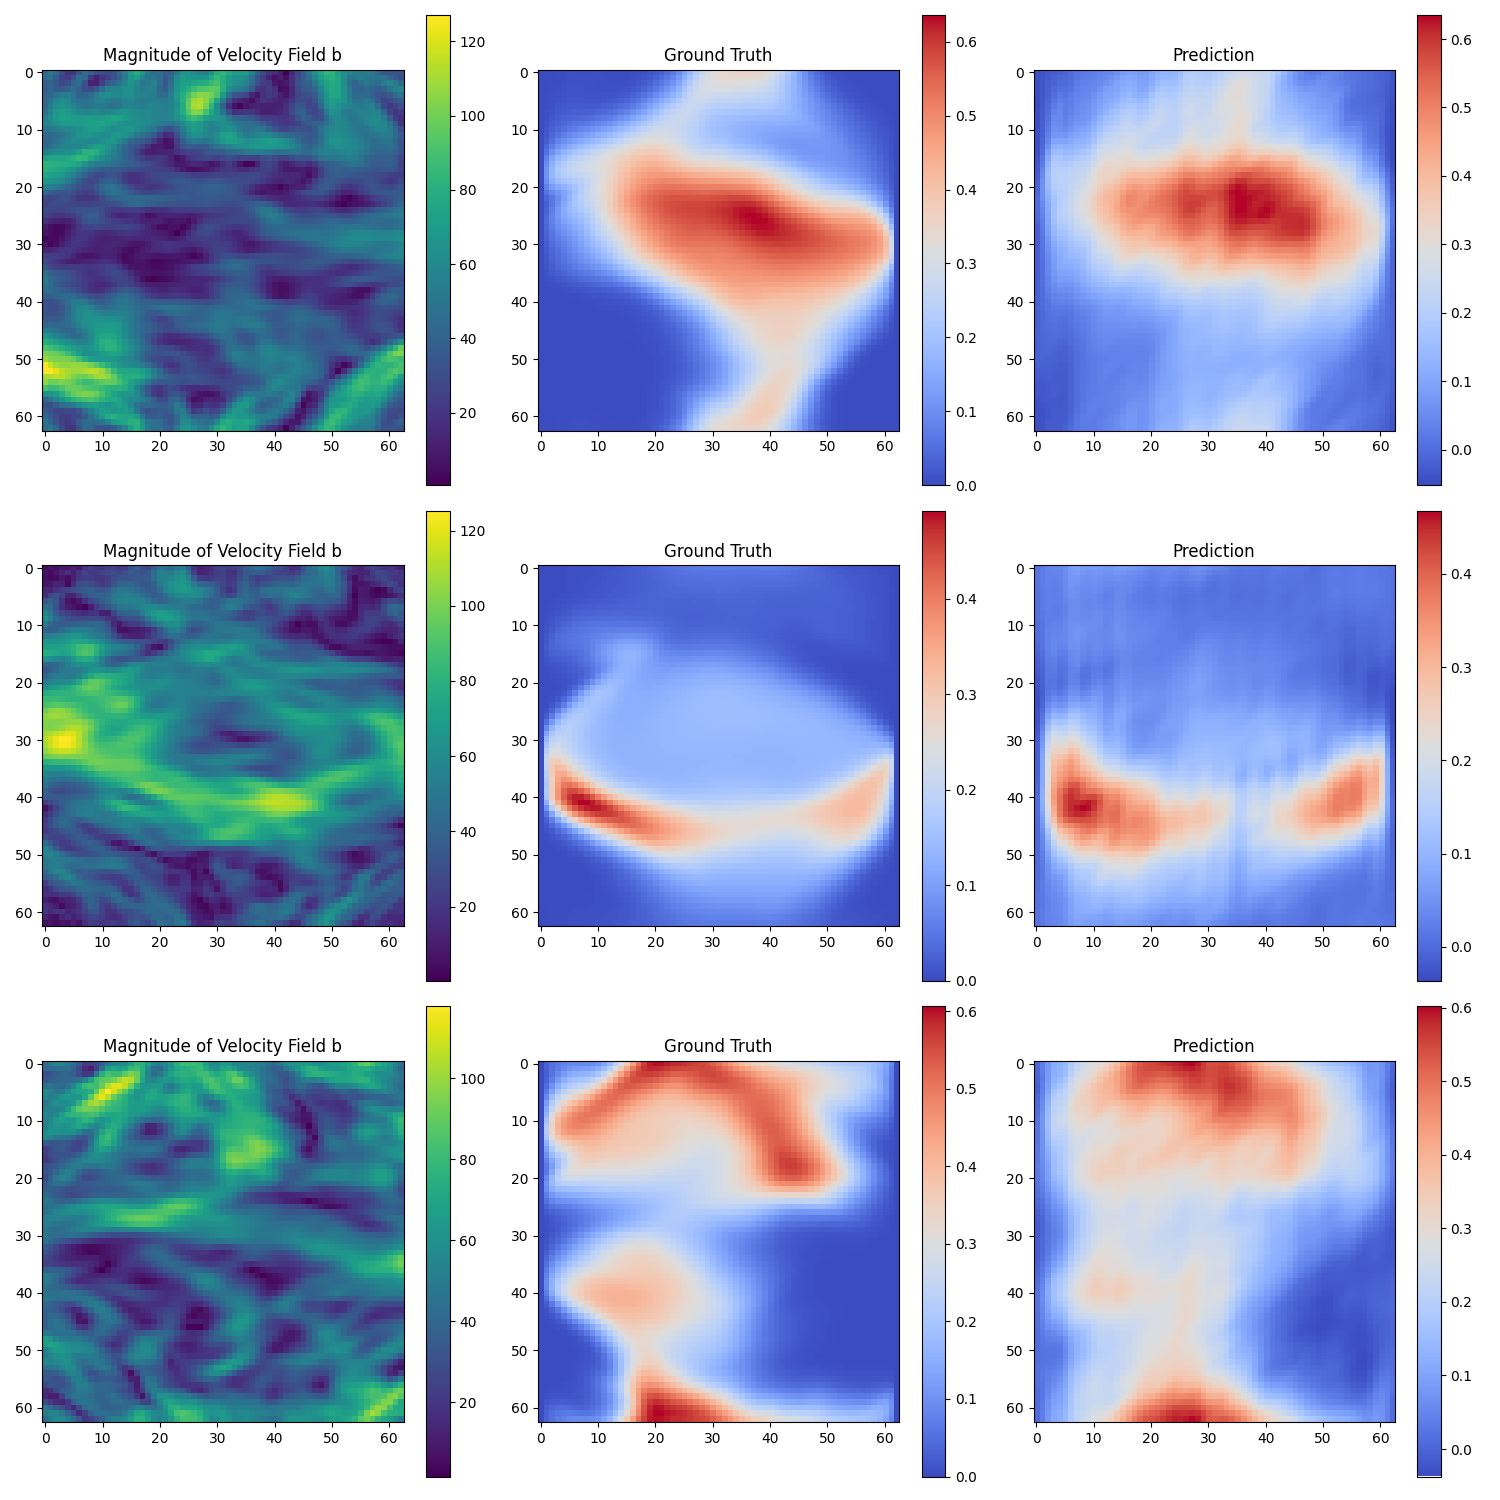
\includegraphics[width=0.7\linewidth]{pred_1.png}
  \caption{Laminar flow testing using FNO}
  \label{fig:laminarflow}
\end{figure}
\bibliographystyle{plain}

\begin {table}[H]
 \caption{Laminar flow performance}
  \label{fig:table6}
\begin{center}
 \begin{tabular}{|c|c|} 
 \hline
& Relative $L^2$ error  \\ [0.5ex] 
 \hline\hline
DeepONet & 0.3376   \\ 
 \hline
FNO & 0.2743    \\ 
 \hline

\end{tabular}
\end{center}
\end {table}

For the second test, we tried a turbulant flow, with the maximum Fourier mode released to 16. The results are shown in Figure \ref{fig:turbulantflow}, and the relative error is shown in table \ref{fig:table7}. 
\begin{figure}[ht]
  \centering
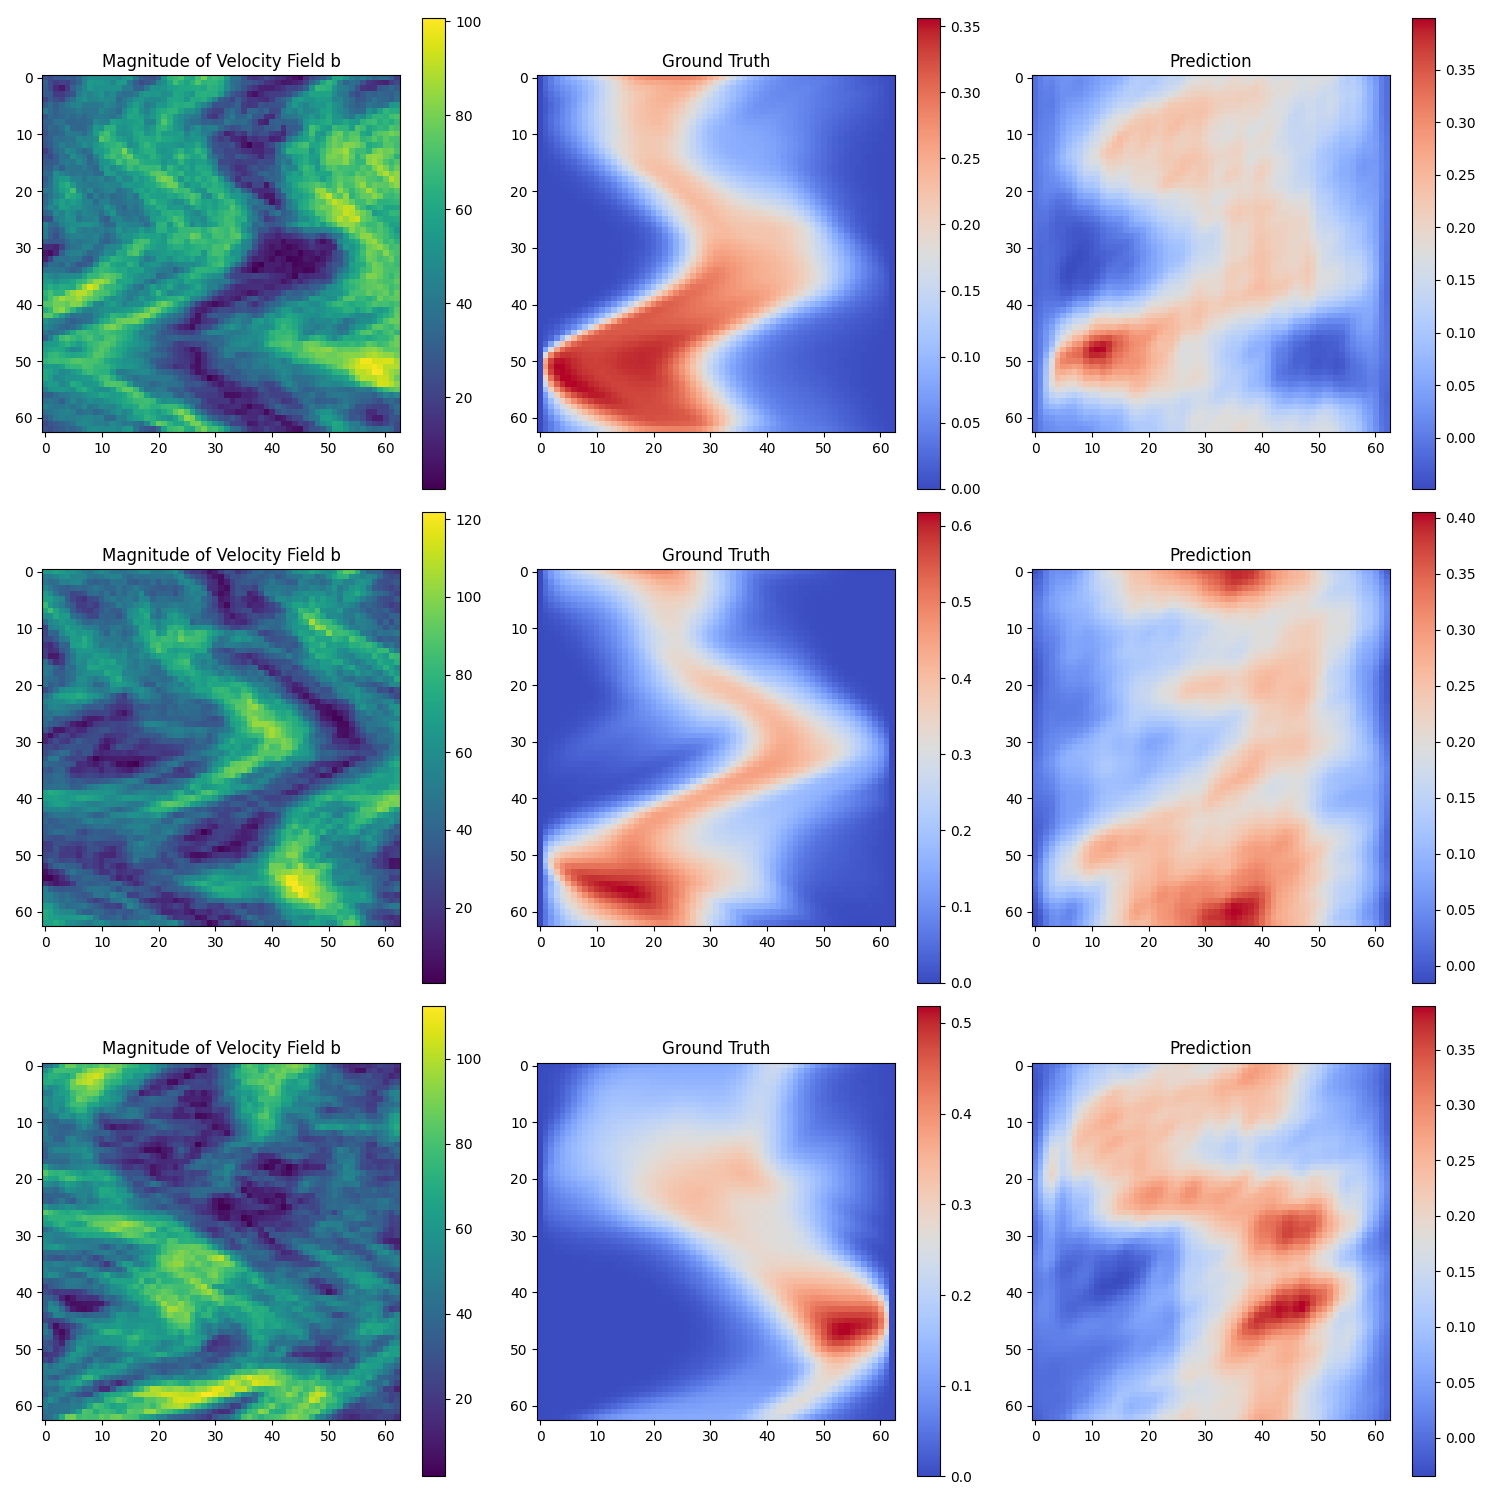
\includegraphics[width=0.7\linewidth]{pred_2.png}
  \caption{Turbulant flow testing using FNO}
  \label{fig:turbulantflow}
\end{figure}
\bibliographystyle{plain}

\begin {table}[H]
 \caption{Turbulant flow performance}
  \label{fig:table7}
\begin{center}
 \begin{tabular}{|c|c|} 
 \hline
& Relative $L^2$ error  \\ [0.5ex] 
 \hline\hline
DeepONet & 0.5138   \\ 
 \hline
FNO & 0.4925    \\ 
 \hline

\end{tabular}
\end{center}
\end {table}

We can see that the relative error is pretty high (around 30\% and 50\%), suggesting that the current setting of nerual operator cannot capture the true flow.

\newpage

\bibliographystyle{plain}

\bibliography{ref}
\end{document}
